
\section{Memory Optimization of Lookaround Oracle}
\label{sec:memory-optimization-oracle}

\subsection{Building the Oracle}

The NFA Simulation can be modified in order to build the oracle for lookbehinds
\cite{systemf_linear_2024} by modifying the \texttt{Accept} instruction
to an instruction that writes to the oracle that it succeeds at the current string
position.

The oracle for a lookahead $r$ can be built in a similar way by considering the NFA
simulation on the regex \texttt{/.*?rev($r$)/} \cite{systemf_linear_2024}. (here, \texttt{rev($r$)}
denotes the regex obtained by reversing the concatenations in $r$, for example for
\texttt{(a|bd)c}, we get \texttt{c(a|db)}). The NFA simulation is then done by reading the input
string backward.

\subsection{Optimizing the Memory}

In order to optimize the memory of the oracle, we will break our string into blocks
of length $K$ (we will be fixing $K$ at the end to minimize the complexity). For
each block, we will not compute the $K$ booleans, but we will instead store the active threads
at the instant before consuming the first character of the block.
\begin{center}
    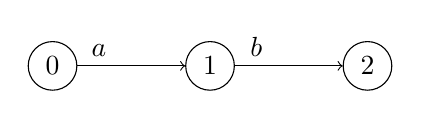
\begin{tikzpicture}
        \node[draw, circle] (root) at (0, 0) {$0$};
        \node[draw, circle] (op1) at (2, 0) {$1$};
        \node[draw, circle] (op2) at (4, 0) {$2$};

        \draw[->] (root) -- node[pos=0.2, above] {$a$} (op1);
        \draw[->] (op1)  -- node[pos=0.2, above] {$b$} (op2);
    \end{tikzpicture} \\ \vspace{0.3ex}
    \begin{tikzpicture}
        \matrix (strmat) [matrix of nodes, ampersand replacement=\&] {
            \texttt{a} \& \texttt{a} \& \texttt{  } \& \texttt{b} \& \texttt{a} \& \texttt{  } \& \texttt{a} \& \texttt{b} \& \texttt{  } \& \texttt{a} \\
        };

        \draw[{Bar[]}-{Bar[]}] ([xshift=-4pt]strmat-1-1.south) -- ([xshift=4pt]strmat-1-2.south);
        \draw[{Bar[]}-{Bar[]}] ([xshift=-4pt]strmat-1-4.south) -- ([xshift=4pt]strmat-1-5.south);
        \draw[{Bar[]}-{Bar[]}] ([xshift=-4pt]strmat-1-7.south) -- ([xshift=4pt]strmat-1-8.south);
        \draw[{Bar[]}-{Bar[]}] ([xshift=-4pt]strmat-1-10.south) -- ([xshift=4pt]strmat-1-10.south);

        \node (it1) at ([yshift=-16pt]strmat-1-1.east) {$\left \{ 0 \right \}$};
        \node (it1) at ([yshift=-16pt]strmat-1-5.west) {$\left \{ 0, 1 \right \}$};
        \node (it1) at ([yshift=-16pt]strmat-1-7.east) {$\left \{ 0, 1 \right \}$};
        \node (it1) at ([yshift=-16pt]strmat-1-10)     {$\left \{ 0, 2 \right \}$};
    \end{tikzpicture} \\ \vspace{0.3ex}
    \textit{Example lookbehind for regex \texttt{ab}, with $K = 2$, for string \texttt{aabaab}. The set of active threads for 
    the instant before consuming the first character of the block is shown below it.}
\end{center}

Whenever the boolean for position $i$ is needed, we will compute the booleans of the entire block
and cache them using the saved starting states for that specific block. We will also discard all the
caches for other blocks so we have at most a single cache at any point in time.

The algorithm is the same for lookaheads, except the active threads stored are the one before consuming the
last character of the block, and reconstruction of the cache is done from the last character of the block
instead of the first.

The memory used per lookaround is therefore $O(K)$ for the cache and $O(|r_i|)$ per block,
where $r_i$ is the regex of the lookaround. There are $|s|/K$
blocks, and so the memory of one lookaround is $O(K + |r_i||s|/K)$. Summing over all lookarounds,
we get $O(|K||r| + |r||s|/K)$, which is minimized when both terms are equal, yielding $K = \sqrt{|s|}$
and a total space complexity of $O(|r| \sqrt{|s|})$.

\subsection{Complexity}

The analysis for the complexity relies on counting the number of time each block will need to be computed.
Let us define $d(r_i)$ to be the depth of the lookaround $r_i$. Here, depth refers to the syntactic
depth if we look at the tree of lookarounds, the main regex has depth $0$, lookarounds inside it have
depth $1$ and lookarounds inside these have depth $2$ etc...

\begin{lemma}
    For a block inside a lookaround of depth $d$, it will be computed at most $d$ times.
\end{lemma}

\begin{proof}
    We will work by induction on the depth, first a lookaround of depth $1$ will only need each
    of its block to be computed at most once. Indeed, the NFA simulation of the main regular
    expression will need the lookaround values in increasing order of string positions, and so
    each block is computed at most once before the cache being cleared to compute blocks of higher
    index.
    
    Now, if we have a lookaround of depth $d + 1$ with one of its block $B_{d+1}$. We consider the parent
    lookaround of depth $d$ with the block $B_d$ aligned with $B_{d+1}$ (since $K$ is a constant
    fixed for all lookarounds in the string). The block $B_{d+1}$ will need to be computed only in $2$ cases,
    either when $B_d$ is computed or when we generate all the active threads for lookaround of depth $d$.
    The first case happens at most $d$ times by induction and the second happens once and is the same as the
    base case as we simulate the full NFA of the lookaround. Thus, block $B_{d+1}$ is indeed computed at most $d + 1$
    times. 
\end{proof}

Using this lemma, we can deduce that every string position and every state in the NFA
will appear in at most $O(D)$ NFA simulations, and so the total time complexity is $O(|r||s|D)$.
